\chapter{Concept}\label{chap:Concept}

\section{The type system}\label{sec:concept:TheTypeSystem}

In \ref{subsec:background:TypeSystems}, we introduce the concept of type systems and we give a brief overview of \textit{type checking} and \textit{type inference}. Our goal is to have solid \textit{application programming interfaces} (APIs) to build type systems for each language.

In this section, we will discuss the importance of the type system for our concept.
What we are looking for in our type system is:
\begin{itemize}
    \item \textbf{modularization}, that allows the definition of custom types and operations on these types, and the ability to combine them in a modular way;
    \item \textbf{flexibility}, since the type system is not known \textit{a priori}, we need the ability to adapt the type system to the specific needs;
    \item \textbf{easy-to-use}, extending the default implementation of the type system with a new type, or implementing a new type from scratch should be easy and straightforward.
\end{itemize}

It is trivial to remember that the type system should also provide the basic functionalities of a type system, such as \textbf{type inference}, that allows the compiler to infer the type of an expression without the need to explicitly specify it; and \textbf{type checking}, that allows the compiler to check if the types of the expressions are correct.

\begin{mydefinition}{type system item}{concept:itemdefinition}
  % this is the text of the theorem. the counter is automatically assigned and,
  % in this example, prefixed with the section number. this theorem is numbered with
  %   \ref{def:concept:itemdefinition} and is given on page \pageref{def:concept:itemdefinition}.
    given that the specifics of the target language for the reference type system are not predetermined (i.e., the language is not known \textit{a priori}), we cannot assume the presence of standard programming constructs such as variables, functions, or objects. therefore, to maintain a broad and adaptable approach, we will use the term \textbf{item} to refer to any of these potential constructs or elements within the system. this ensures that our discussion remains relevant regardless of the particular features and paradigms of the target language.
\end{mydefinition}

\subsection{type: the basic building block}\label{subsec:concept:typethebasicbuildingblock}

The \textbf{Type} is the basic building block of the type system. It is used to represent the type of an expression, such as a variable, a function, or an object. The \textbf{Type} can be a primitive type, such as \textit{int}, \textit{float}, \textit{string} or a custom type, such as a \textit{class}, \textit{interface}, or \textit{enum}.

\begin{mydefinition}{Type}{concept:type}
The name \textbf{type} could be misleading because it does not exactly represent the type of an item but rather it is class of types that allows to build a specific type of a given category. Note that, this is not excluing that each concreate type could have a specific (class of) \textbf{type}, but defining a \textbf{type} as a class of types allows to define a generic \textbf{type} for all the types of a given category (i.e., all primitive types) and defining once the operations that can be performed on them.
\end{mydefinition}

In our concept, during the implementation of the type system, several types will be defined. Each type will have a set of operations that can be performed on it. In abstract terms, we can define a type as a set of operations that can be performed on it.
Basically, each type should be answer to the following questions:
\begin{enumerate}
    \item What is its \textbf{identifier}?
    \item Can it be \textbf{assignable from} another type with a specific kind of \textbf{variance}?
    \item Can it match a specific \textbf{signature}?
    \item Does it need other types to be \textbf{bound}?
\end{enumerate}

The second question is used to \textbf{type check} the \textit{item} in the \textbf{Type System}. The type of \textbf{variance} is used to define the relationship between two types. The variance can be \textit{covariant}, \textit{contravariant}, or \textit{invariant}.

\begin{definition}{Variance}\\
    Suppose $A$ and $B$ are types, and $I[U]$ denotes application of a type constructor I with type argument $U$. Within the type system of a programming language, a typing rule for a type constructor $I$ is:
    \begin{itemize}
        \item covariant if it preserves the ordering of types ($\leq$), which orders types from more specific to more generic: If $A \leq B$, then $I[A] \leq I[B]$;
        \item contravariant if it reverses this ordering: If $A \leq B$, then $I[B] \leq I[A]$;
        \item bivariant if both of these apply (i.e., if $A \leq B$, then $I[A] \equiv I[B]$);
        \item variant if covariant, contravariant or bivariant;
        \item invariant or nonvariant if not variant.
    \end{itemize}
\end{definition}

The third question is used to \textbf{type inference} the \textit{item} in the \textbf{Type System}, simply answering to the question: can the type of the \textit{item} match a specific \textbf{signature}?
Finally, the last question is used to \textbf{bind} the type to its generic parameters. For example, the type \textit{List<String>} is bound to the type \textit{List<T>} with \textit{needed types} being \textit{String}.


\subsection{Scope: the context of the type}\label{subsec:concept:ScopeTheContextOfTheType}

\begin{mydefinition}{Scope}{concept:scope}
The \textbf{Scope} is the context in which an identifier is defined, more precisely, where the binding between the type and an identifier is defined in the \textbf{Type System}. It is used to define the visibility and the lifetime of the identifier and its operations. The \textbf{Scope} can be, for example, a \textit{local scope}, a \textit{global scope}, or a \textit{module scope}.
\end{mydefinition}

In our concept, a \textbf{Scope} can be see as a \textbf{Type}~\ref{subsec:concept:typethebasicbuildingblock} that defines the visibility and the lifetime of the type or identifier and its operations. At this point, the \textbf{Scope} is not universal. In fact, for instance, \textit{Java} do not categorize the \textbf{Scope}, such as \textit{Block Scope}, as a \textbf{Type}. However, in order to achieve a representation of a \textit{Block Scope} as a \textbf{Type}, we can define a \textbf{Scope} where at the questions

\begin{itemize}
    \item Can it be assignable from another type with a specific kind of variance?
    \item Can it match a specific signature?
\end{itemize}

will answer \textit{false}.

So, a \textbf{Scope} should be able to answer to the following questions, in addition to the questions that a \textbf{Type} should be able to answer:

\begin{enumerate}
    \item What types are \textbf{visible} in the \textbf{Scope}?
    \item Can a type be bound to an identifier in the \textbf{Scope}?
    \item If exists, what is the \textbf{parent Scope}?
    \item Can a \textbf{Scope} be marked as \textbf{external visible} and what items exported?
\end{enumerate}

The first question is used to define the visibility of the type in the \textbf{Scope} and knowing what types are visible in the \textbf{Scope}.~\ref{subsec:concept:TypingEnvironmentTheSymbolTable} will be used to answer this question.
The second question is used to bind a type to the Scope. Every scope should have a set of rules that allow to determine if a type can be bound to the Scope.~\ref{subsubsec:concept:EntryTypeBinderAnHelperToBindTypes} will be used to answer this question.
The third question is used to define the hierarchy of the Scopes. Trivially, this is represented as a tree.
Finally, the last question is used to define the visibility of the Scope and its items. A \textbf{Scope} marked as \textit{external visible} should be able to export some its items. This is useful during \textit{type inference} phase, because whan searching for a type if a Scope (type) is marked as \textit{external visible} the search should be performed recursively in all \textbf{items} exported by the \textbf{Scope}.

Now, we propose some examples of scopes in the world of object-oriented programming (OOP) languages.
In OOP there are several types of scopes that determine the visibility and lifetime of items. The most common scopes are:
\begin{itemize}
    \item \textbf{Class scope}:  A class is a collection of variables and methods. Variables declared inside a class have class scope, and they can be accessed within that class and its instances. Methods declared inside a class also have class scope and can be accessed within that class and its instances.
    \item \textbf{Instance scope}: An instance is an object created from a class. Instance variables are declared inside a class, but outside any method, and have instance scope. They can be accessed within that class’s methods and any instance of that class.
    \item \textbf{Method scope}: Variables declared inside a method have method scope, and they can only be accessed within that method.
    \item \textbf{Block scope}: A block is a section of code enclosed in curly braces. Variables declared inside a block have block scope, and they can only be accessed within that block. This includes loops, conditional statements, and code enclosed in curly braces.
    \item \textbf{Static scope}: Static variables and methods belong to a class, not to an instance of that class. Static variables and methods have class scope and can be accessed using the class name without creating an instance of the class.
\end{itemize}

\subsection{Signature: the definition of the type}\label{subsec:concept:SignatureTheDefinitionOfTheType}

A \textbf{Signature} is the definition of the type. It is used to define the structure of the type and to support \textit{static typing} and \textit{type checking}. In our type system, \textbf{each type} should have a Signature that defines the structure of the type.

\begin{mydefinition}{Signature}{concept:signature}
    The \textbf{Signature} in \textbf{structural type system}~\cite{Cardelli88, Cook89} or in \textbf{nominal type system}~\cite{Pierce02} is the definition of the type. In a \textbf{structural type system}, the \textbf{Signature} is the structure of the type, while in a \textbf{nominal type system}, the \textbf{Signature} is the name of the type. The \textbf{Signature} is used also to support \textit{static typing} and \textit{type checking}.
\end{mydefinition}

A \textbf{structural type system} is a major class of type systems in which type compatibility and equivalence are determined by the type's actual structure or definition and not by other characteristics such as its name or place of declaration. A type system is \textbf{nominal} if compatibility and equivalence of data types is determined by explicit declarations and/or the name of the types.

A \textbf{Signature} should be able to answer to one question:

\begin{enumerate}
    \item Can a type match the \textbf{Signature}?
    \item Can I resolve the type of an identifier from the \textbf{Signature}?
\end{enumerate}

Answering to this question can be simple or complex, depending on the type we would like to match with the \textbf{Signature}. For example, a type can be a primitive type, such as \textit{int}, \textit{float}, \textit{string}, or a custom type, such as a \textit{method} inside a \textit{class}.
For instance, a \textbf{Signature} is often used to define the type of a function. In this case, the \textbf{Signature} is the definition of the function in terms of its parameters and return type.
Usually, every \texttt{Type} should have a \texttt{Signature} that defines the structure of the type.
Additionally, to perform \textit{type inference}, the \textbf{Signature} is used to infer the type of an expression.

\subsection{Symbol Table Entry: an entry in the Typing Environment}\label{subsec:concept:SymbolTableEntryAnEntryInTheTypingEnvironment}

A \textbf{Symbol Table Entry} is an entry in the \textbf{Typing Environment} (Symbol Table). It is used to store a informations associated to a symbol in the \textbf{Type System}.

\begin{mydefinition}{Symbol}{concept:symbol}
    A \textbf{Symbol} is a name that represents a value, a variable, a function, or any other item in a program. In the \textbf{Type System}, a \textbf{Symbol} is used to represent a type, a variable, a function, or any other item in the program.
    Usually, symbols are collected during the \textit{parsing} phase of the compilation process and stored in a \textbf{Symbol Table}.
    A symbol can be a \textit{nonterminal symbol} or a \textit{terminal symbol}. A \textit{nonterminal symbol} is a symbol that can be expanded into other symbols, while a \textit{terminal symbol} is a symbol that cannot be expanded further.
\end{mydefinition}


The \textbf{Symbol Table Entry} should be able to answer, at least, to the following questions:
\begin{enumerate}
    \item What is the \textbf{Type} of of the associated symbol?
    \item What is the \textbf{Kind} of of the associated symbol?
    \item What is the \textbf{Location} of of the associated symbol?
    \item What are the \textbf{Details} of of the associated symbol?
\end{enumerate}

As one can guess, the \textbf{Symbol Table Entry} is used to store the information associated with a symbol in the \textbf{Type System}.
Note that to answer the first question, the \textbf{Symbol Table Entry} should have a \textbf{Type} associated with it. The answer to the second question of~\ref{subsec:concept:SignatureTheDefinitionOfTheType} can help to infer the \textbf{Type} of the associated symbol if the \textbf{Type} is not explicitly defined.
The second question is used to define the \textbf{Kind} of the associated symbol. The \textbf{Kind} can be, for example, a \textit{declaration}, a \textit{definition}, a \textit{use} or an \textit{import}.
The third question is used to define the \textbf{Location} of the associated symbol. The \textbf{Location} can be, for example, a \textit{line number} or a \textit{column number}.
Finally, the last question is used to define the \textbf{Details} of the associated symbol. The \textbf{Details} can be, for example, a \textit{description} or \textit{extra information} about the symbol.

\subsubsection{Entry Type Binder: an helper to perform type binding}\label{subsubsec:concept:EntryTypeBinderAnHelperToBindTypes}

The \textbf{Entry Type Binder} is an helper to perform type binding in the \textbf{Type System}. It is used to bind a type to an identifier in the \textbf{Scope}.
The \textbf{Entry Type Binder} should be able to answer to the following questions:
\begin{enumerate}
    \item Is this identifier already bound to the \textbf{Scope}?
    \item Can I bind an identifier to a \texttt{SymbolTableEntry} in this \textbf{Scope}?
\end{enumerate}

The first question is used to determine if the identifier is already bound to the \textbf{Scope}. If the identifier is already bound to the \textbf{Scope}, the \textbf{Entry Type Binder} should return an error.
The second question is used to determine if the identifier can be bound to a \texttt{SymbolTableEntry} in the \textbf{Scope}. If the identifier can be bound to a \texttt{SymbolTableEntry} in the \textbf{Scope}, the \textbf{Entry Type Binder} should bind the identifier to the \texttt{SymbolTableEntry}.

\subsection{Typing Environment: the symbol table}\label{subsec:concept:TypingEnvironmentTheSymbolTable}

The \textbf{Typing Environment} is the symbol table in the \textbf{Type System}. It is used to store the information associated with the symbols in the \textbf{Type System}.
Basically, the \textbf{Typing Environment} is a map between symbol or identifier and \texttt{SymbolTableEntry}.

The \textbf{Typing Environment} should be able to answer to the following questions:
\begin{enumerate}
    \item What are the symbols in the \textbf{Typing Environment}?
    \item Can I get the \texttt{SymbolTableEntry} associated with a symbol in the \textbf{Typing Environment}?
    \item Can I add a symbol to the \textbf{Typing Environment}?
    \item Can I remove a symbol from the \textbf{Typing Environment}?
\end{enumerate}

In section~\ref{subsec:concept:ScopeTheContextOfTheType}, we defined the \textbf{Scope}. Combining the \textbf{Scope} with the \textbf{Typing Environment}, we can define the visibility of the types in the \textbf{Scope} and the lifetime of the types in the \textbf{Scope}.
Answering to the first question, the \textbf{Typing Environment} should be able to return the symbols in the \textbf{Typing Environment}; it it like answering to the question: what are the types or identifiers visible in the \textbf{Scope}?
The second question is used to get the \texttt{SymbolTableEntry} associated with a symbol in the \textbf{Typing Environment}. This is useful to get the information associated with the symbol.
The third question is used to add a symbol to the \textbf{Typing Environment}. This is useful to add a new symbol to the \textbf{Scope}.
Finally, the last question is used to remove a symbol from the \textbf{Typing Environment}. This is useful to remove a symbol from the \textbf{Scope}.

In Figure~\ref{lst:concept:type_system}, we have a final representation of the type system.

\begin{figure}[tbh]
    \centering
    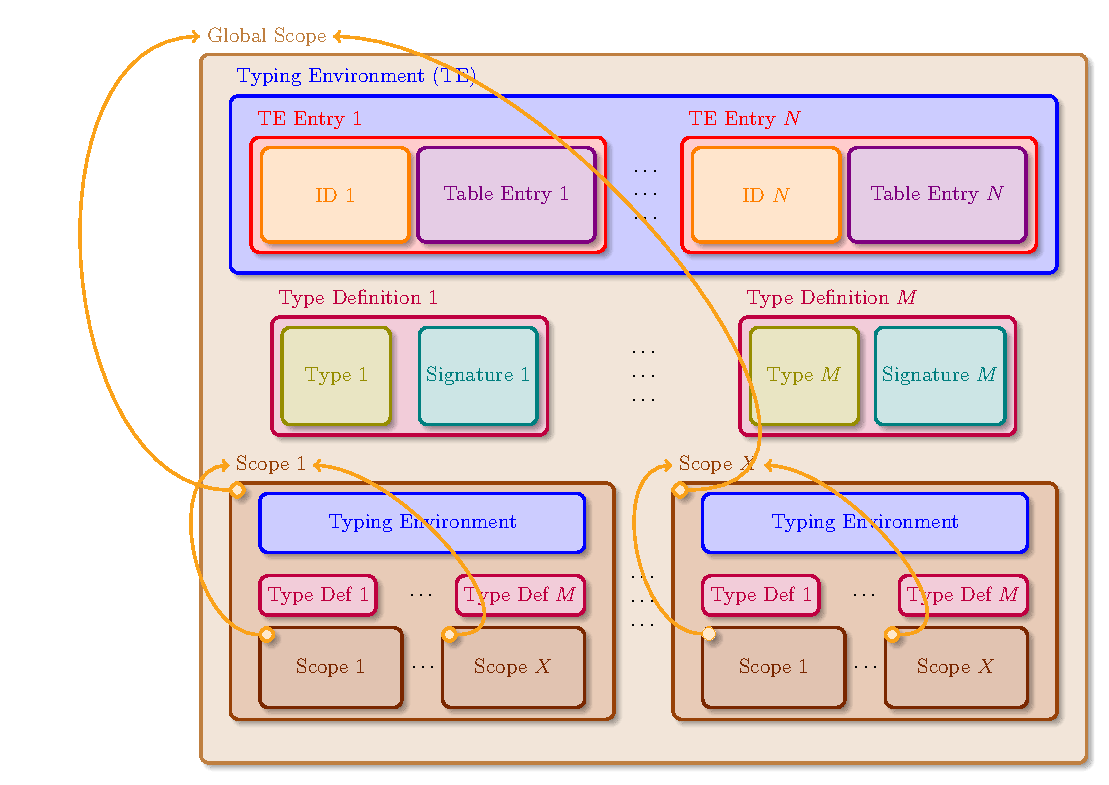
\includegraphics[width=0.9\linewidth]{figs/concept/type_system.pdf}
    \caption{A final representation of the type system}
    \label{lst:concept:type_system}
\end{figure}

\subsection{Type Inference: the ability to infer the type of an expression}\label{subsec:concept:TypeInferenceTheAbilityToInferTheTypeOfAnExpression}

As already mentioned in~\ref{subsubsec:background:TypeInferenceInProgrammingLanguages}, \textbf{Type Inference} is the ability to infer the type of an expression without the need to explicitly specify it. It is used to determine the type of an expression based on the context in which it appears.
In our concept, \textbf{Type Inference} is used to infer the type of an expression in the \textbf{Type System}.
The \textbf{Type Inference} should be able to answer to the following questions:
\begin{enumerate}
    \item Can I infer the type of an expression?
    \item Can I resolve the type of an identifier from the \textbf{Typing Environment}?
\end{enumerate}

The first question is used to determine if the type of an expression can be inferred. If the type of an expression can be inferred, the \textbf{Type Inference} should infer the type of the expression. The second question is used to resolve the type of an identifier from the \textbf{Typing Environment}. This is useful to infer the type of an expression based on the context in which it appears.

There are multiple algorithms to perform \textbf{Type Inference}, such as \textit{Hindley-Milner}~\cite{Hindley69, Milner78}, \textit{unification-based}~\cite{Robinson65}, and \textit{constraint-based}~\cite{Pierce02} algorithms. In our concept, we will use a \texttt{Strategy Pattern} to define the \textbf{Type Inference} algorithm.
In order to perform \textbf{Type Inference}, we should have a list of all possibile candidates for the type of the expression. This list creation is performed by the \textbf{Type Lookup} algorithm~\ref{alg:typelookup}.

\begin{algorithm}[h]
\caption{Pseudocode to show how type lookup is performed\label{alg:typelookup}}
\begin{algorithmic}
\Require $I$ identifier, $SIG$ signature, $S$ scope
\Ensure$L$ list of all candidates
\State $L\gets\emptyset$ \Comment{Initialize $L$ with an empty list}
\State $CS \gets S$
\While{$CS \neq \emptyset$}
\ForEach {$Type$ in $CS$ with identifier $I$}
\If {$Type$ match signature $SIG$}
\State $L \gets L\cup\{Type\}$
\EndIf
\EndFor
\State $CS \gets$ parent of $CS$ \Comment{parent could be $\emptyset$}
\EndWhile
\State\Return $L$
\end{algorithmic}
\end{algorithm}

\subsection{Example: a simple C program}\label{subsec:concept:ExampleASimpleCProgram}

Now, we propose an example where putting all the concepts together. In Listing~\ref{lst:concept:Example}, we have a simple C program that defines a global variable \texttt{const\_one} and a function \texttt{main} that prints (using the \texttt{printf} function) the value of the variable \texttt{const\_one} and the value of the variable \texttt{two}.

\begin{Listing}[tbh]
    \centering
    \showc*[0.75\textwidth]{Example.c}
    \caption{Example of a simple C program}
    \label{lst:concept:Example}
\end{Listing}

After parsing the program, the \textbf{Typing Environment} should contain the following information:

\begin{table}[t]
    \rowcolors{2}{gray!25}{white}
    % \setlength\arrayrulewidth{0pt}
    \centering
    \begin{tabular}{ c c c c c c }
        \toprule  \textbf{Scope} & \textbf{Identifier} & \textbf{Type} & \textbf{Kind} & \textbf{Location} & \textbf{Details} \\
        \midrule
        \textbf{Global} & \texttt{stdio.h} & \texttt{header} & \texttt{import} & \texttt{1:1 - 1:18} &  \\
        \textbf{Global} & \texttt{const\_one} & \texttt{int} & \texttt{declaration} & \texttt{3:11 - 3:19} & \texttt{const} \\
        \textbf{Global} & \texttt{main} & \texttt{function} & \texttt{declaration} & \texttt{5:5 - 5:8} &  \\
        \textbf{main} & \texttt{two} & \texttt{int} & \texttt{declaration} & \texttt{6:9 - 6:11} & \\
        \textbf{main} & \texttt{printf} & \texttt{function} & \texttt{use} & \texttt{7:5 - 7:10} & \texttt{external} \\
        \textbf{main} & \texttt{const\_one} & \texttt{int} & \texttt{use} & \texttt{7:25 - 7:33} &  \\
        \textbf{main} & \texttt{+} & \texttt{function} & \texttt{use} & \texttt{7:35 - 7:35} &  \\
        \textbf{main} & \texttt{two} & \texttt{int} & \texttt{use} & \texttt{7:37 - 7:39} &  \\
        \bottomrule
    \end{tabular}
    \caption{Language Workbenches Supporting Modularization, Composition and Precompiled Features}
    \label{tab:concept:Example}
\end{table}

\begin{itemize}
    \item The \texttt{stdio.h} header is imported in the \textbf{Global Scope}.
    \item The \texttt{const\_one} variable is declared in the \textbf{Global Scope} as a constant integer.
    \item The \texttt{main} function is declared in the \textbf{Global Scope}.
    \item The \texttt{two} variable is declared in the \texttt{main Scope} as an integer.
    \item The \texttt{printf} function is used in the \texttt{main Scope} and is marked as external.
    \item The \texttt{const\_one} variable is used in the \texttt{main Scope}.
    \item The \texttt{+} operator is used in the \texttt{main Scope}.
    \item The \texttt{two} variable is used in the \texttt{main Scope}.
\end{itemize}

Note that in table~\ref{tab:concept:Example}, we have the \textbf{Scope} as first column, but in reality, is the \textbf{Scope} that defines the visibility and the lifetime of the types in the \textbf{Typing Environment}. In fact, in our explanation in section~\ref{subsec:concept:ScopeTheContextOfTheType}, we defined the \textbf{Scope} as the context in which an identifier is defined, more precisely, where the binding between the type and an identifier is defined in the \textbf{Type System}. So, ideally, every \textbf{Scope} should have a \textbf{Typing Environment} associated with it.
As we can see, these information will be used also to perform the \textbf{modularization} of the LSP (see section~\ref{sec:concept:TowardsAModularTypeSystem}).


\section{Towards a modular type system}\label{sec:concept:TowardsAModularTypeSystem}

In this section, we will discuss the importance of having a modular type system. In particular, we will focus on the ability to define types and operations on these types in a modular way and the ability to combine them.
In the context of language workbenches, the ability to define types and operations on these types in a modular way is crucial. In fact, the language workbenches should be able to support different languages and paradigms, and the ability to define types and operations on these types in a modular way is crucial to achieve this goal.

The \textbf{modularization} of the type system is important for several reasons:
\begin{itemize}
    \item \textbf{Reusability}: The ability to define types and operations on these types in a modular way allows to reuse the types and operations in different contexts.
    \item \textbf{Extensibility}: The ability to define types and operations on these types in a modular way allows to extend the types and operations with new types and operations.
    \item \textbf{Flexibility}: The ability to define types and operations on these types in a modular way allows to adapt the types and operations to the specific needs.
\end{itemize}

In the context of language workbenches and Language Product Lines (SPLs), we are trying to aswer to the following research questions:
\begin{itemize}
    \item[RQ1] How can we define types and operations on these types in a modular way?
    \item[RQ2] How can we combine types and operations on these types in a modular way?
    \item[RQ3] Can we achieve the type checking and type inference in a modular way?
\end{itemize}

Thus, everything we have seen so far is very abstract, in the following sections we will see how the following APIs are adapted to an AST.

Consider the simple JavaScript program in Listing~\ref{lst:concept:sum}, which defines two functions to sum two numbers.
\begin{Listing}[tbh]
    \centering
    \showjs*[0.9\textwidth]{sum.js}
    \caption{A simple JavaScript program that defines two functions to sum two numbers.}
    \label{lst:concept:sum}
\end{Listing}

The AST of the program in Listing~\ref{lst:concept:sum} is shown in Figure~\ref{lst:concept:ast_sum}.
\begin{figure}[t]
    \centering
    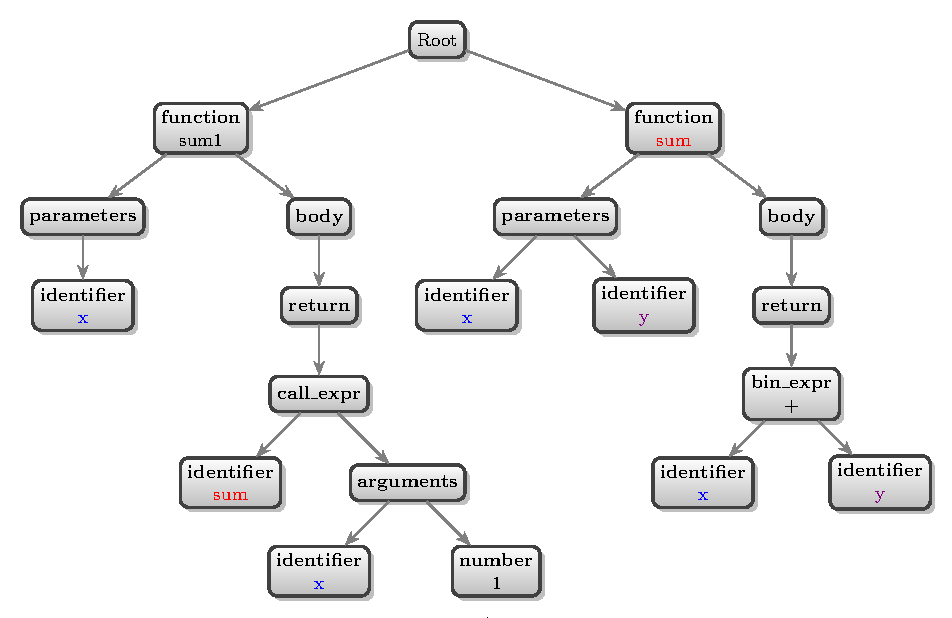
\includegraphics[width=0.9\linewidth]{figs/concept/simple_ast.pdf}
    \caption{AST of source code~\ref{lst:concept:sum}.}
    \label{lst:concept:ast_sum}
\end{figure}

\subsection{Compilation Unit: a logical unit of source code}\label{subsec:concept:CompilationUnitALogicalUnitOfSourceCodeo}

Usually, a \textbf{compilation unit} is a logical unit of source code that is processed by the compiler as a single entity. It typically consists of a single source code file and any header files that it includes. In some programming languages, such as C and C++, each compilation unit (also kwown as translation unit) must have a unique name and can contain multiple functions or variables. Other programming languages, such as Java~\cite{javacompilationunits},  use a different approach where each compilation unit corresponds to a single class definition.

\begin{mydefinition}{compilation unit}{concept:compilationunit}
    In this particular concept, a \textbf{compilation unit} is responsibile for a specific portion of the code, which includes a set of subtrees within the abstract syntax tree (AST). It is responsible for traversing the nodes of the AST that pertain to its assigned portion through a compilation unit task (see more~\ref{subsec:concept:CompilationUnitTaskATaskToPerformCompilation}). Additionally, it serves as a supportive tool for semantic actions, where the compilation unit is utilized to execute detailed analysis for performing certain actions, as explained in further detail below.
\end{mydefinition}

The operations for which a compilation unit is used are:
\begin{itemize}
    \item \textbf{enter or leave a scope}, when a new compilation unit is created, it has a stack with a scope that represents the initial scope.
        \begin{itemize}
            \item when \textit{entering} a scope it is pushed onto the stack and the old scope becomes the parent of the new scope (e.g. when transitioning from a global scope to a function scope, the global scope becomes the parent of the function scope. This enables all the entities that exist within the global scope to still be inferred from the function scope).
            \item when \textit{exiting} the current scope is popped from the stack.
        \end{itemize}
    \item \textbf{bind an identifier to an entity} on the current scope
    \item perform \textbf{type inferences} on the current scope
\end{itemize}

There are several actions that are performed during the traversal of the AST.
Supposing we have the AST~\ref{lst:concept:ast_sum}, the sequence of events during its preorder traversal would be as follows:
\begin{enumerate}
    \item creating a new compilation unit with \texttt{global} scope as initial
    \item binding a new function with identifier \textit{sum1} in the current scope
    \item entering in scope of the function \textit{sum1}
    \item \label{itm:ast-node-eval} evaluating ast node \textit{params} and \textit{body}
    \item exit from scope of the function \textit{sum1} and returning inside global scope
    \item binding a new function with identifier \textit{sum} in the current scope
    \item entering in scope of the function \textit{sum}
    \item evaluating ast node \textit{params} and \textit{body}
    \item exit from scope of the function \textit{sum} and returning inside global scope
\end{enumerate}
When the body of the sum1 function (\inlinejs{return sum(x,1)}) is evaluated at point 4, it will performed the following operations:
\begin{itemize}
    \item infer the type of x and 1
    \item and then infer the type of sum given type of x and type of 1 as signature
\end{itemize}

In the first case the inference is \textbf{successful} because $x$ has been defined before (in the ast node params) and $1$ is a primitive type known a priori in this case it will be up to the developer to find a way to store the entities that make up the base of the language.

On the other hand, the inference of the $sum$ type \textbf{fails} because the relevant node, which defines the function, has not yet been visited.
To address this issue, two potential solutions are available:
\begin{itemize}
    \item one option is to mandate that users define functions before using them, potentially through the introduction of concepts similar to C function prototypes,
    \item another solution involves altering the order of visits, ensuring that all functions are defined before entering their respective bodies.
\end{itemize}
The choice that was made to maintain the flexibility of the API was to modify the visit order of the AST, the next section explains how the visit order is managed.


\subsection{Compilation Unit Task: a task to perform compilation}\label{subsec:concept:CompilationUnitTaskATaskToPerformCompilation}

As discussed in the earlier section, the preorder visit approach may encounter challenges when trying to infer types that have not been defined yet. To address this issue, the programmer can determine the order of node visitation. This allows the option to either visit a node immediately or create a compilation unit task that will execute the visit only when authorized (further details to follow).

The programmer has the flexibility to determine the sequence of node visits in the following ways:
\begin{itemize}
    \item  Immediate node visit: The programmer can choose to visit other nodes without delay.
    \item Compilation unit task creation: The programmer can create a compilation unit task that visits associated nodes only when permitted.
\end{itemize}

These operations can coexist, allowing the programmer to visit certain nodes immediately while deferring others as compilation unit tasks. Each task has its own dependency and priority, which are crucial factors in determining the execution order. For instance, while at node "function sum1" in tree~\ref{lst:concept:ast_sum}, the programmer can opt to visit the "params" node right away, while creating a compilation unit task for the "body" node.

The programmer specifies points in the code where a compilation unit task is created, enabling deferred traversal of specific nodes in the Abstract Syntax Tree (AST). To ensure smooth traversal, the compilation unit task must adhere to the following properties:
\begin{itemize}
    \item It must be associated with exactly one Compilation Unit.
    \item Multiple unit tasks cannot visit the same node simultaneously.
    \item Each task can only be executed once during compilation.
\end{itemize}

Remarking, each compilation unit task must be associated with a single compilation unit, meaning that whenever a task is created, a corresponding compilation unit must also be created.

\begin{figure}[t]
    \centering
    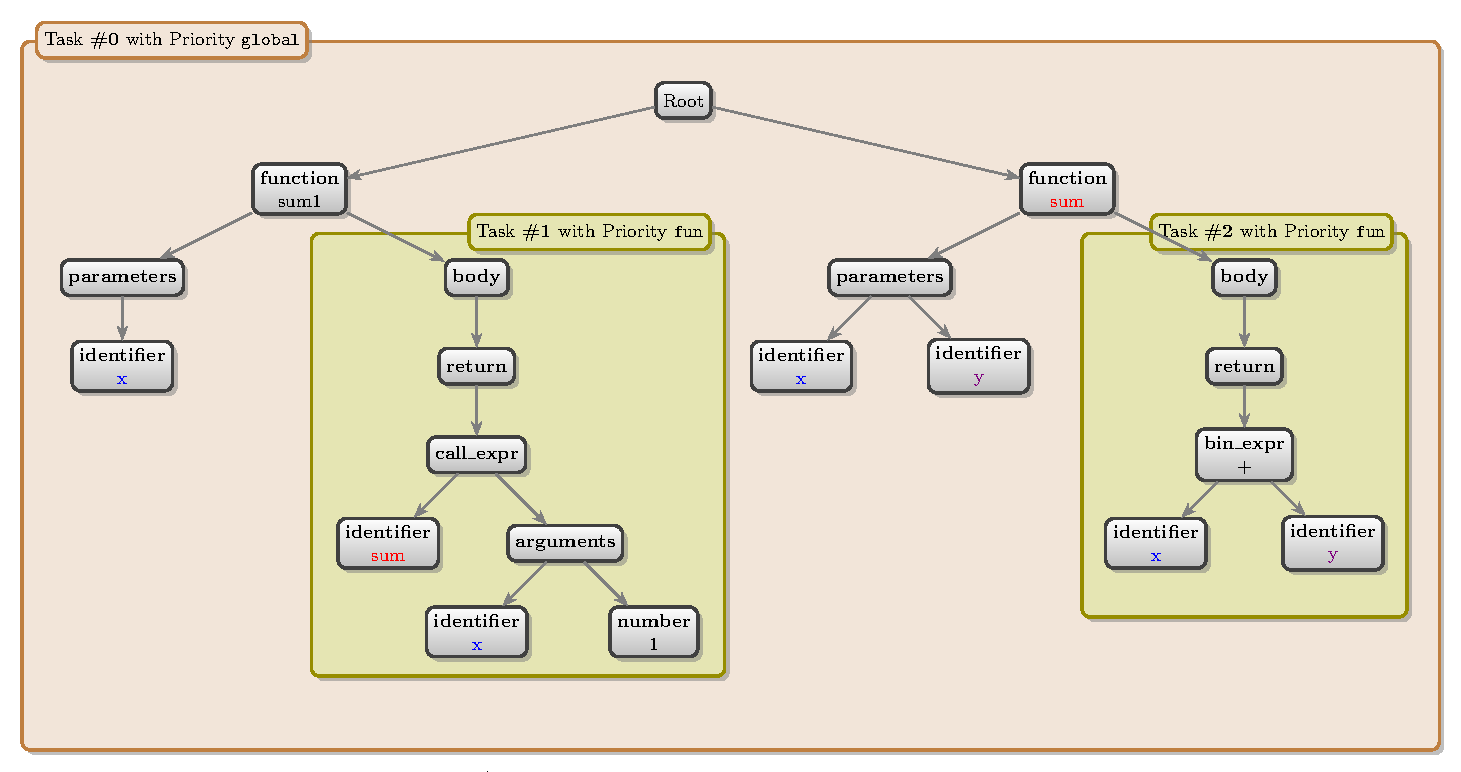
\includegraphics[width=0.9\linewidth]{figs/concept/simple_ast_annotated.pdf}
    \caption{AST with \textbf{task} and \textbf{priority} annotations.}
    \label{lst:concept:ast_sum_annotated}
\end{figure}

After introducing the concept of a compilation unit task, the visit order of the AST nodes can be reviewed as follows (see figure~\ref{lst:concept:ast_sum_annotated}):

\begin{enumerate}
    \item When the root node is visited, a task (\#0) associated with the root of the AST node is created.
    \item Task \#0, when executed, performs a preorder visit of the children nodes (function sum1 and function sum). The only difference compared to before (the visit done in~\ref{lst:concept:ast_sum}) is that the body node is not executed immediately. Instead, another task is created for the body node, which will be executed subsequently.
    \item Tasks \#1 and \#2 are executed only after task \#0 has finished, ensuring that the inference of "sum" can be correctly performed because it happens after the definition of the function "sum".
\end{enumerate}

However, the method for managing the order of task execution has not been clarified yet. In the next section, we will discuss how this will be accomplished.

\subsection{Compilation Helper: an helper to perform compilation}\label{subsec:concept:CompilationHelperAnHelperToPerformCompilation}

A compilation unit is associated with a piece of code, whereas a compilation helper is shared among all the compilation phases. The compilation helper is responsible for creating and registering new compilation units, along with their associated tasks. Later, the registered tasks can be executed by the compilation helper.

\subsubsection{Root type and root compilation unit}

To initialize the compilation helper, it is required to define a root type that represents the global scope of the entire source set being compiled. Using this global scope, the compilation unit root is created, and its associated task will be the first one to be executed.

\subsubsection{Hooks}

Compilation Helper provides the capability to define custom hooks that are executed at specific phases during the execution process.
The available hooks currently include:

\begin{itemize}
    \item \inlinejava{beforeAll}: which is executed prior to the initialization of all roots
    \item \inlinejava{beforeEach}: which is executed before the initialization of each individual root in every file
\end{itemize}
These hooks can be easily implemented by overriding the default methods provided by the Compilation Helper.

\subsubsection{Task creation}

In order to generate a task, it is imperative to establish a compilation unit.
When you are creating a compilation unit the following situations can arise:
\begin{itemize}
    \item \textit{Creating a new scope}: This necessitates the generation of a new compilation unit that is linked to the newly created scope.
    \item \textit{Utilizing the current scope}:
    \begin{itemize}
        \item If the current scope is the root scope, the root task is updated with additional nodes to visit.
        \item If the current scope is not the root, a fresh compilation unit is generated.
    \end{itemize}
\end{itemize}
When a new compilation unit is generated, a corresponding task is also created with two key pieces of information: its dependency and execution priority. In our case, each task is dependent on the task from which it was generated, ensuring that it is executed only after its parent task has completed. The execution priority is a class \inlinejava{T} that extends \inlinejava{Comparable<T>}, allowing for custom prioritization of tasks.

Both the dependency and priority information are utilized by the executor to effectively manage the order in which the tasks are executed, as we will see in the next section.
\begin{algorithm}[h]
\caption{The algorithm used for compilation task execution}\label{alg:executor}
\begin{algorithmic}
\Require $X$ list of all prioritized tasks
\While{$X \neq \emptyset$}
\State $N \gets$ collect tasks with highest priority in $X$
\State $X \gets X \setminus N$
\State create a DAG from $N$
\State execute the DAG \Comment{DAG execution could populate $X$ with new tasks}
\State wait for completion
\EndWhile
\end{algorithmic}
\end{algorithm}

\subsubsection{Task execution}

The tasks are executed following the algorithm shown in ~\ref{alg:executor}.
Tasks that are independent of each other can run in parallel.

\subsection{A family of type systems}\label{subsec:concept:AFamilyOfTypeSystems}
In the context of language workbenches and Software Product Lines (SPLs), the modularization of type systems enables the creation of a family of type systems. This is particularly advantageous for supporting various languages and paradigms. By constructing the type system in a modular fashion, each component or "artifact" of the type system can be activated or deactivated as needed, resulting in a tailored type system for specific language requirements. This section explores how such modularity facilitates flexibility, reusability, and extensibility in language development.

\subsubsection{Modular Type Systems in Language Workbenches}

Language workbenches aim to provide tools and frameworks to define and manipulate programming languages. One of the core aspects of a language is its type system, which encompasses the rules and operations for type checking and type inference. A modular type system allows the language designer to define these rules and operations in separate, interchangeable modules.

\noindent \textbf{Key Benefits}:
\begin{itemize}
    \item \textbf{Reusability}: Modular type systems enable the reuse of type definitions and operations across different languages and contexts. For example, a module that defines numeric types and arithmetic operations can be reused in multiple languages without modification.
    \item \textbf{Extensibility}: New types and operations can be added to the system without altering the existing modules. This is particularly useful in evolving languages or when creating domain-specific languages (DSLs) that require specialized types.
    \item\textbf{ Flexibility}: Modules can be selectively activated or deactivated, allowing for the customization of the type system to meet specific needs. This is essential for supporting multiple paradigms or language variants within the same framework.
\end{itemize}

\noindent \textbf{Language Product Lines (LPLs)}

In SPLs, the concept of modular type systems aligns with the idea of product families. Each "product" in the line can be seen as a specific configuration of the language, with certain type system features enabled or disabled.
Creating a Family of Type Systems

\begin{itemize}
    \item \textbf{Type System Artifacts}: Each component of the type system (such as type definitions, type checking rules, and type inference mechanisms) is treated as an artifact. These artifacts can be independently developed, maintained, and combined.
    \item \textbf{Configuration Management}: The language workbench provides mechanisms to manage configurations, allowing language designers to specify which artifacts are included in a particular language instance. This can be achieved through configuration files, annotations, or a graphical interface.
    \item \textbf{Dependency Management}: Dependencies between artifacts are managed to ensure that the activation of one artifact automatically includes any required dependencies. For instance, enabling a type inference module may also require certain type definitions to be included.
    \item \textbf{Dynamic Activation}: During compilation or interpretation, the system dynamically activates the relevant type system artifacts based on the configuration. This allows the same underlying infrastructure to support different language features as needed.
\end{itemize}

\noindent Example: Type Checking and Inference in Action

Consider a scenario where a language product line includes multiple variants of a programming language, each with different type-checking requirements. One variant might require strict type checking for all variables, while another might allow more lenient type inference for certain constructs. Using a modular type system, these variants can be configured by selectively activating the appropriate type-checking and inference modules.

For instance, the type-checking module for strict type enforcement can be activated for the strict variant, ensuring that all variables must be explicitly typed. In contrast, the lenient variant can activate a module that implements type inference rules, allowing the system to deduce types where explicit annotations are missing. Additionally, common modules that handle basic type definitions and generic type operations can be shared across both variants, promoting reuse and reducing redundancy.

\section{The relevance of the type system in the LSP design}\label{sec:concept:RelevanceOfTheTypeSystem}

The type system is the core of the LSP design. We illustrate the need of having a type system by focusing on the ability to respond to requests from a \textit{Language Client}.

In the reminder of this section, we will evaulate the relevance for three of the most important LSP feautre introduced in \ref{subsec:bacground:KeyMethodsOverview}.

\subsubsection{Diagnostic Analysis}\label{subsubsec:concept:DiagnosticAnalysis}

Currently, the LSP provides the ability to perform \textit{diagnostic analysis} on the code. This feature is useful to provide feedback to the user about the correctness of the code.
In compilers design, a \textit{Diagnostic} can be produced by different phases of compilation, such as the \textit{lexical analysis}, \textit{syntax analysis}, and \textit{semantic analysis}.
The \textbf{Syntax Errors} are detected by the \textit{lexical analysis} and \textit{syntax analysis}, usually during the \textit{parsing} phase. The \textbf{Semantic Errors} are detected by the \textit{semantic analysis}, usually during the \textit{type checking} phase.
In modern compilers, an additional phases can be added to the compilation process, \textit{data flow analysis} and \textit{control flow analysis}, that can be used to detect more complex errors, such as \textit{unreachable code} or \textit{dead code}.

In Language Workbenches world, usually it is common to have an instance of a \textbf{Language} and a \textbf{Source Code} that should be parsed and analyzed by the Language.
Taking into account the \textbf{Syntax Errors}, assuming that the \textbf{Language} is able to parse the \textbf{Source Code} and the \textbf{Language} is able to provide errors and warnings during the \textit{parsing} phase, should be easy to provide the \textit{Syntax Errors} to the \textit{Language Client} (see Listing \ref{lst:concept:SyntaxError}).

\begin{Listing}[t]
    \centering
    \showjava*[1\textwidth]{SyntaxError.java}
    \caption{Example of catching a Syntax Error in Java}
    \label{lst:concept:SyntaxError}
\end{Listing}

The \textbf{Semantic Errors} and \textbf{Data Flow Analysis} are more complex to implement. In fact, in order to detect a \textit{Semantic Error}, the \textbf{Language} should be able to perform \textit{type checking} on the \textbf{Source Code} in order to verify that the code can be executed without any unexpected errors. The \textit{Data Flow Analysis} is necessary to understand if the code is reachable, and to do this, the \textbf{Language} should be able to perform static analysis on the \textbf{Source Code}.

\subsubsection{Jump to Definition}\label{subsubsec:concept:JumpToDefinition}
The ability to access the definition of a symbol, such as a function or a variable, is a common feature in modern IDEs.
To enable this functionality, a \textbf{Symbol Table} is required and should be able to map a given row and column position in the source code to the corresponding symbol and its definition.
During this phase, the typechecking is required to bind the symbol to its type. This is necessary to provide the correct definition of the symbol to the user.
In addition to the symbol table, the \textbf{Language} should be able to provide the \textit{Scope} of the symbol, in order to understand if the symbol is visible in the current context.

\subsubsection{Code Completion}\label{subsubsec:concept:CodeCompletion}

To effectively handle this kind of request, such as the one depicted in figure~\ref{fig:completion}, the language server needs to comprehend the type of symbol for which suggestions are to be provided. Once the type is determined, returning relevant suggestions becomes straightforward. However, a challenge arises when suggestions must be presented to the user while they are still writing, as the source code may be syntactically incorrect during the writing process. To address this issue, a parser with error detection and recovery~\cite{Graham79} capabilities is required to enable effective suggestion generation despite the presence of syntax errors.


\section{LSP: a modular approach}\label{sec:concept:LSPAModularApproach}

LSP and DAP are protocols that describes a common \textit{Application Programming Interface} (API) that the \textbf{language server} (LS) should implement, with the benefit of having only one implementation of the LS and multiple clients (IDEs and SCEs) that can consume it, essentially establishing a \textit{client-server} relationship through a communication channel (e.g., \textit{pipes} or \textit{sockets}).
However, the implementation of an LS and its integration with an IDE/SCEs is still a complex task, as it requires the knowledge of the LSP specification and the implementation of the language support.
The implementation~\cite{Gunasinghe22} of an LS is done entirely manually and it is a \textit{top-down} activity, where most of the time is spent on the design and implementation data structures and algorithms.
Since 1990s~\cite{Kang90}, researchers have started talking about the \textit{Software Product Lines} (SPLs) \cite{Cazzola23d, Cazzola20} to move towards a more modular world, where the implementation of a software system can be done in a compositional way, by composing the features of the SPL.
When a SPL is applied to the implementation of a programming language, each product corresponds to a language variant \cite{Cazzola15f} taking the name of \textit{Language Product Lines} (LPLs) \cite{Cazzola15f}. LPLs have been successfully used in both GPLs \cite{Cazzola16, Cazzola16i, Cazzola15f} and DSLs \cite{Haugen08, Cazzola14e, White09}.
\begin{figure}[t]
    \centering
    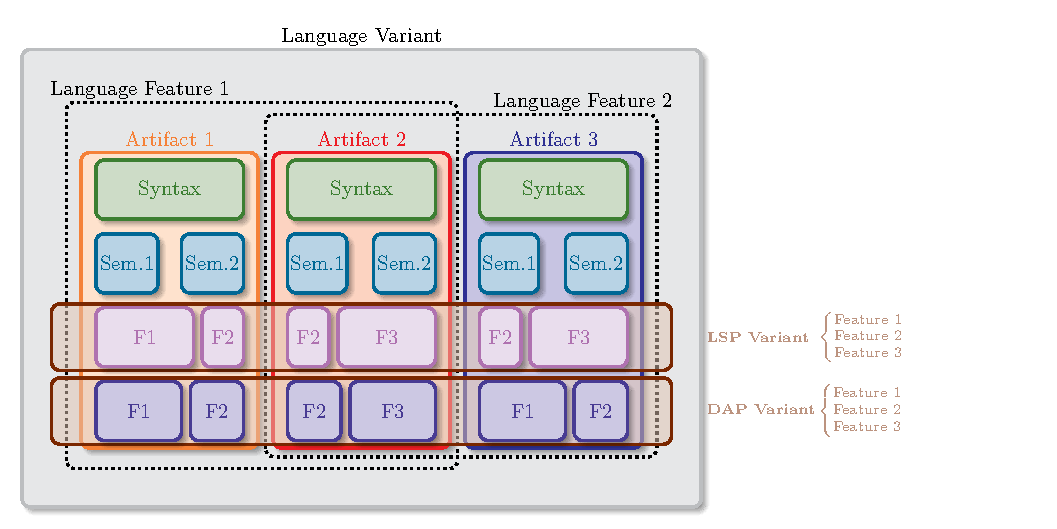
\includegraphics[width=0.9\linewidth]{figs/concept/module_with_lsp.pdf}
    \caption{Proposed approach to modular implementation of LSP and DAP.}
    \label{lst:concept:module_with_lsp}
\end{figure}

What I want to prove with this thesis is that the implementation of an LS could be a \textit{bottom-up} activity, where each LSP or DAP functionality can be seen as a separate \textit{feature module} \cite{Batory04, Kastner11} splitted across the language artifacts, where each artifacts can be part of one or more \textit{language features} (see Figure~\ref{lst:concept:module_with_lsp}). These units can be composed to provide a modular implementation of the LS. This approach is supported by the fact that the LSP and the DAP are \textit{language-agnostic} protocols~\cite{Niephaus20, Rodriguez-Echeverria18} (see Fig.~\ref{lst:lsp}), which means that it does not impose any restrictions on the implementation of the LS, as long as it respects the specification of the protocol.
In \textit{feature-oriented programming} (FOP) \cite{Apel13, Czarnecki04, Prehofer01}, a feature module is a unit of composition that encapsulates a specific functionality, and it is a first-class entity that can be composed with other feature modules to form a software system; similar to an aspect module that encapsulates a crosscutting concern in \textit{aspect-oriented programming} \cite{Kiczales01, Kiczales97, Laddad03}. Using FOP in language development, a family of languages~\cite{Liebig13} can be defined by composing feature modules~\cite{Wende09}, and a language can be seen as a product of the family.
In this way, the implementation of the LS is a \textit{bottom-up} activity, where each artifact has attached a part of LSP and DAP feature module that implements the LS functionality for that \textit{language fragment}, and these units can be composed to provide a modular implementation having \textbf{variants} of the LS.

\subsection{Index Tree}\label{subsec:concept:IndexTree}

\begin{algorithm}[tbh]
    \caption{The algorithm used to get a symbol from IndexTree}\label{alg:lookup}
    \begin{algorithmic}
        \Require $(row, col)$ a position on the file, $N$ the node of the index tree
        \Ensure A set of SymbolTableEntry entries
        \State $S \gets$ the SymbolTableEntry entry associated with $N$
        \If{$(row, col)$ is within the selection range of $N$}
        \State \Return $\{S\}$
        \ElsIf{$(row, col)$ is within the folding range of $N$}
        \ForEach {$C$ in $N$'s children}
        \State $Result\gets$call this algorithm with $(row, col)$ and $C$
        \If {$Result$ is not empty}
        \Return $Result$
        \EndIf
        \EndFor
        \Else
        \State \Return $\emptyset$
        \EndIf
    \end{algorithmic}
\end{algorithm}

The Index Tree is a sophisticated data structure specifically designed to store and manage information about the source code, such as symbols, types, and references. This structure is pivotal for Language Servers (LS) to efficiently provide essential features like "Jump to Definition" and "Code Completion." Its design facilitates rapid and accurate symbol location based on their positions within a text file, making it an integral component of modern code editors and development environments. In figure~\ref{lst:conept:lsp_combinations}, we illustrate the structure of the Index Tree and its key components; as example, we consider the source code in Listing~\ref{lst:concept:sum}.

\begin{figure}[t]
    \centering
    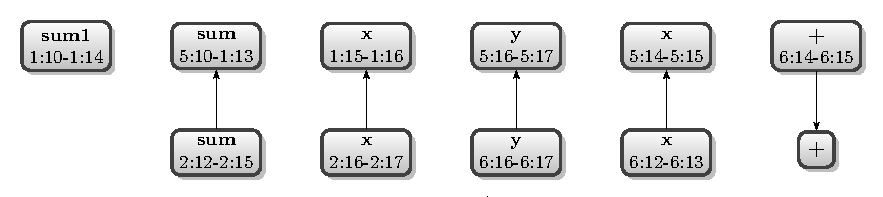
\includegraphics[width=0.9\linewidth]{figs/concept/index_tree.pdf}
    \caption{Index Tree structure for the source code in Listing~\ref{lst:concept:sum}.}
    \label{lst:conept:lsp_combinations}
\end{figure}


The Index Tree is structured as follows:
\begin{itemize}
    \item \textbf{Nodes and SymbolTableEntry:} Each node in the Index Tree is represented by a \texttt{SymbolTableEntry}. This entry encapsulates all relevant information about a particular symbol in the source code, including its type, position, and references.
    \item \textbf{Internal Nodes and Folding Range:} Internal nodes in the tree must possess a folding range. This range is a continuous segment within the source code that encompasses all the symbols contained within the node. The folding range ensures that related symbols are grouped together logically.
    \item \textbf{Selection Range:} The selection range refers to the exact range within a node that contains a specific symbol. It is more precise than the folding range and is used for pinpointing the location of a symbol within the node.
\end{itemize}

The Index Tree supports several critical functionalities for the Language Server:
\begin{itemize}
\item \textbf{Efficient Symbol Search:} The tree structure allows for straightforward symbol searches. Given a position in the text file, the tree can be traversed to locate the corresponding node, thanks to the hierarchical organization of folding ranges and selection ranges.
\item \textbf{Jump to Definition:} By leveraging the Index Tree, the Language Server can quickly locate the definition of a symbol when a user invokes the "Jump to Definition" feature.
\item \textbf{Code Completion:} The tree also aids in code completion by providing a structured and easily navigable repository of all symbols and types within the source code.
\end{itemize}

One of the key advantages of the Index Tree is its modularity:

\begin{itemize}
    \item \textbf{Language-Specific Populations:} The tree is populated by the specific programming language, meaning each language can add its own symbols, types, and references to the tree.
    \item \textbf{Composition with Other Features:} The Index Tree serves as a foundational component that can be composed with other language features. This modular approach allows for a more flexible and scalable implementation of the Language Server, enabling it to support a wide range of languages and features.
\end{itemize}

The efficiency of the Index Tree lies in its hierarchical structure and the way it organizes symbols within ranges. The time complexity for inserting a symbol into the tree or searching for a symbol generally depends on the depth of the tree. In the average case, both operations can be expected to run in \(O(\log n)\) time, where \(n\) is the number of symbols in the source code. This logarithmic complexity ensures that the Index Tree can handle large codebases efficiently, providing quick access to symbols even as the size of the source code grows.

In summary, the Index Tree is a highly efficient and modular data structure that plays a crucial role in modern Language Servers. Its ability to store and organize symbols, types, and references, combined with its efficient search and retrieval capabilities, makes it an indispensable tool for providing advanced code navigation and completion features.

\subsection{Symbol Dependency Graph}\label{subsec:concept:SymbolDependencyGraph}

The symbol dependency graph serves as a vital data structure within the language server framework, designed to interconnect symbols in a manner that facilitates efficient responses to client queries. In essence, it's a graph where nodes represent SymbolTableEntry instances, and edges are annotated with labels denoting the type of relationship. Currently, the primary relationship label is "usage," indicating that one symbol uses another.

This graph plays a crucial role in several key functionalities of the language server:

\begin{itemize}
    \item \textbf{Calculating Symbol References}: By traversing the graph, the server can determine all references to a specific symbol throughout the codebase. This is essential for tasks like finding where a symbol is used or referenced.
    \item \textbf{Navigating to Symbol Definitions}: Utilizing the graph, the server can pinpoint the exact location within the code where a symbol is defined. This capability is crucial for enabling developers to quickly navigate to the declaration of a symbol.
\end{itemize}

\subsubsection{Diagnostic Handling}\label{subsubsec:concept:DiagnosticHandling}
During the parsing and static analysis phases, the language server gathers diagnostics, which are issues or potential problems identified in the code. These diagnostics are collected and presented to the client at the end of compilation. Custom diagnostics can be registered through exceptions or specialized data structures like \textbf{TypesystemException} or \texttt{LogRecord}.

\subsubsection{Definition, References, and Hover Features}\label{subsubsec:concept:DefinitionReferencesAndHoverFeatures}

When a user requests information about a specific position in a file—such as the definition, references, or details on hover—the server follows these steps:

\begin{itemize}
    \item \textbf{Index Tree Lookup}: Using an index tree, the server identifies the symbol associated with the requested position, if it exists.
    \item \textbf{Graph Traversal}: For definition and reference queries, the server traverses the symbol dependency graph to retrieve all relevant definitions or references of that symbol. This traversal is guided by the relationships defined in the graph.
    \item \textbf{Hover Information}: For hover queries, the server executes methods annotated with @Hover to provide detailed contextual information about the symbol at the specified position.
\end{itemize}

\subsubsection{Document Symbol, Semantic Token, Inlay Hint, and Folding Range}\label{subsubsec:concept:DocumentSymbolSemanticTokenInlayHintAndFoldingRange}

These capabilities involve listing and presenting symbols and structural elements within a file:

\begin{itemize}
    \item \textbf{Document Symbol}: Lists all symbols present in a file using the index tree.
    \item \textbf{Semantic Token}: Provides structured information about tokens in the code for language-specific operations.
    \item \textbf{Inlay Hint}: Displays subtle UI hints, annotations, or metadata within the editor.
    \item \textbf{Folding Range}: Enables collapsing and expanding regions of code based on predefined folding ranges associated with symbols.
\end{itemize}

\subsubsection{Additional Capabilities}\label{subsubsec:concept:AdditionalCapabilities}
Other functionalities, though not implemented by default, can be achieved by leveraging data structures obtained during static analysis. These capabilities include advanced tasks such as semantic analysis, type checking, and code optimization, which benefit from the comprehensive understanding of code structure and dependencies provided by the symbol dependency graph.

In summary, the symbol dependency graph is pivotal in enabling precise navigation, comprehensive symbol analysis, and the delivery of rich contextual information within the language server ecosystem. Its structured representation of symbol relationships forms the backbone for many essential IDE features, enhancing developer productivity and code comprehension.

\section{A \textit{modular} DSL for semplifying the LSP and type system development}\label{sec:concept:AModularDSLForSemplifyingTheLSPAndTypeSystemDevelopment}

\begin{Listing}
\begin{bnf*}
  \bnfprod{program}
    {\bnfpn{type definition} \bnftd{*} \bnfpn{scope definition} \bnftd{*}  \bnfpn{type inferencing} \bnftd{*}}\\
    \bnfmore{\bnfpn{type checking} \bnftd{*} \bnfpn{error catching} \bnftd{*}}\\
    \bnfmore{\bnfpn{generic op} \bnftd{*}}\\
  \bnfprod{type definition}
    {\bnfts{define } \bnfpn{type definition or} \bnftd{ [} \bnfpn{callback} \bnftd{]}}\\
  \bnfprod{scope definition}
    {\bnfts{define scope } \bnfpn{scope} \bnfpn{nlg token} \bnftd{ [} \bnfpn{range} \bnftd{]}}\\
  \bnfprod{range}
    {\bnfts{from } \bnfpn{nlg term} \bnfts{ to } \bnfpn{nlg t} \bnftd{ [} \bnfpn{priority} \bnftd{]}}\\
  \bnfprod{priority}
    {\bnfts{[ run } \bnfpn{nlg nt} \bnfts{ priority } \bnfpn{scope} \bnftd{ [} \bnfpn{callback} \bnftd{]} \bnfts{ ]}}\\
  \bnfprod{callback}
    {\bnfts{ then } \bnfpn{callback}}\\
  \bnfprod{type definition or}
    {\bnfpn{nlg type} \bnfpn{nlg token} \bnfor \bnfpn{type} \bnfpn{nlg token}}\\
  \bnfprod{type inferencing}
    {\bnfts{infer } \bnfpn{signature} \bnfts{ : } \bnfpn{nlg token}} \bnftd{ [} \bnfpn{type inferencing opt} \bnftd{]}\\
  \bnfprod{type inferencing opt}
    {\bnfts{=> } \bnfpn{nlg type} \bnfor \bnfts{with [} \bnfpn{nlg type} \bnfts{*]}}\\
  \bnfprod{type checking}
    {\bnfts{check } \bnfpn{nlg token} \bnfts{ : } \bnfpn{nlg type} \bnfpn{variance} \bnfpn{nlg type}}\\
  \bnfprod{generic op}
    {\bnfts{enter scope} \bnfor \bnfts{exit scope} \bnfor \bnfts{initRoot}}\\
  \bnfprod{error catching}
    {\bnfts{try \{ } \bnfpn{program} \bnfts{ \}} \bnftd{ [} \bnfts{on } \bnfpn{nlg exeption}  \bnfts{ \{ } \bnfpn{program} \bnfts{ \}} \bnftd{]}}\\
  \bnfprod{variance}
    {\bnfts{covariant} \bnfor \bnfts{contravariant} \bnfor \bnfts{invariant}}\\
  \bnfprod{nlg token}
    {\bnfpn{nlg nt} \bnfts{.token}}\\
  \bnfprod{nlg type}
    {\bnfpn{nlg nt} \bnfts{.type}}\\
  \bnfprod{nlg nt}
    {\bnfts{\$} \bnfpn{digit}}\\
  \bnfprod{nlg t}
    {\bnfts{\#} \bnfpn{digit}}\\
  \bnfprod{digit}
    {\bnfts{[0-9]}}\\
  \bnfprod{scope}
    {\bnftd{the name of the scopes defined in the language}}\\
  \bnfprod{type}
    {\bnftd{the name of the types defined in the language}}\\
  \bnfprod{signature}
    {\bnftd{the name of the signatures defined in the language}}\\
  \bnfprod{callback}
    {\bnftd{the name of the callbacks defined in the language}}
\end{bnf*}
  \caption{Grammar for the TypeLang DSL.}
  \label{lst:concept:typelang_grammar}
\end{Listing}

\begin{Listing}
    \centering
    \showneverlang*[1\textwidth]{FunDeclaratationJava.nl}
    \caption{A Neverlang module that defines a function declaration.}
    \label{lst:concept:fun_declaration_java}
\end{Listing}


In Section~\ref{subsec:concept:CompilationUnitTaskATaskToPerformCompilation}, we discussed effective techniques for managing the traversal of an Abstract Syntax Tree (AST) in code. Listing~\ref{lst:concept:fun_declaration_java} provides a concrete example of how the semantic action linked to the production for the declaration of a javascript function can be implemented. The portion enclosed in \texttt{0.{}.} corresponds to the semantic action associated with the FunDeclaration node. When the AST in Y is referenced, this code is executed when the sum1~\ref{lst:concept:sum} function is visited.

Key points about this code include the following: Lines 27-39 detail the creation of a new symbol table entry for the function identifier symbol, which is associated with the TypeFunction type; a specific implementation of the Type interface. In lines 31-47, a new task is registered to visit the body of the function when executed. Lines 51-51 involve evaluating the params node within the scope of the newly created function. In line 53, a TypesystemException exception is caught and forwarded on a shared communication channel, confining the error to a specific code region and allowing the AST visit to continue.

Further explanation of the code is typically unnecessary, as programmers usually write Java code using a Domain-Specific Language (DSL) called TypeLang for ease of use. Upcoming sections will provide detailed information on the functionalities of this DSL.


Every terminal symbol can be used as an identifier. In addition to the associated string, the token also contains the position of the identifier, given by the URI of the file and the range of the token. To create a token from a Neverlang nonterminal, use the syntax \texttt{Token.fromASTNode(n, 0)}, where 0 represents the index of the nonterminal, corresponding to \texttt{\#0} in Neverlang-stylish syntax.

The basics of grammar and documentation are outlined in Listing~\ref{lst:concept:typelang_grammar}, which lists all the constructs that make up TypeLang.
The provided grammar defines various constructs and operations related to type binding, type scoping, task definition, callback execution, type inferencing, and type checking within a hypothetical language or system. The goal of this grammar is to facilitate the creation and management of types, tasks, and error handling in a structured and automated way.

The first set of rules deals with type binding. By using \texttt{define \$1.type \$2.token}, we establish a new type binding where the content of the \texttt{\$2} token attribute becomes the identifier, and the content of the \texttt{\$1} type attribute is the type. Additionally, \texttt{define \$1 \$2} translates to \texttt{\$1.type \$2.token} by default, allowing for more straightforward type binding definitions. The rule \texttt{define customType \$2.token} optionally adds a token attribute for custom types, indicating flexibility in how types are defined.

Next, the grammar introduces the concept of type scope definition. By defining \texttt{scope module \$1.token}, a new type scope module is bound to the token of \texttt{\$1}. This scope is further elaborated by \texttt{define scope module \$1.token from \#0 to \#1}, which sets a folding range from \texttt{\#0} to \texttt{\#1}. This range likely indicates the span within the source code where this scope is applicable.

In the context of task definition, the rule \texttt{define scope module \$1.token from \#0 to \#1} followed by \texttt{[ run \$1 priority module ]} specifies a new compilation unit task. This task is designed to visit node \texttt{\$1} with the priority set to \texttt{module}. The inclusion of square brackets denotes the encapsulation of the task definition within a specific scope and range.

Callbacks are handled through two primary rules. The first, \texttt{define customType \$2.token then customCallback}, ensures that a callback function named \texttt{customCallback} is executed at the end of binding a custom type. The second rule, \texttt{define scope module \$1.token from \#0 to \#1 [ run \$1 priority module then customCallback ]}, integrates a callback execution at the end of a task, ensuring custom behavior post-task execution.

Type inferencing rules provide mechanisms to infer types based on specific signatures and tokens. The rule \texttt{infer customSignature \$1.token} infers a type with a signature named \texttt{customSignature} and token \texttt{\$1.token}. Furthermore, \texttt{infer customSignature \$1.token => \$1.type} stores the inferred type in \texttt{\$1.type}. The rule \texttt{infer function \$1.token with [\$1 \$2]} infers a function type, passing \texttt{\$1.type} and \texttt{\$2.type} as parameters to the function constructor signature.

Type checking ensures that types remain consistent. The rule \texttt{check \$0.token : \$0.type is invariant \$1.type} verifies that \texttt{\$0.type} remains invariant when compared to \texttt{\$1.type}, using \texttt{\$0.token} for error location purposes. This step is crucial for maintaining type safety and correctness in the system.

Lastly, error catching is handled similarly to the try-catch construct in general-purpose languages (GPLs). The grammar provides a structure for capturing and managing exceptions, ensuring that any caught errors are submitted to \texttt{CompilationHelper} for processing. This error management framework is essential for robust and reliable system behavior, allowing for graceful handling of unexpected issues during compilation or execution.

In summary, this grammar provides a comprehensive framework for defining and managing types, scopes, tasks, callbacks, type inferencing, type checking, and error handling. Each production rule contributes to a structured approach to system design, ensuring type safety, task prioritization, and robust error management.

Additionally, TypeLang generates code automatically based on the type system of the target language, ensuring that each DSL adheres to its own type system. For instance, the statement \texttt{define customType $1 $2} can be parsed only if the user has associated the keyword customType with a class extending Type. This association is established using the annotations, as documented in Listing~\ref{lst:concept:typelang_annotations}.

We are able to use two different kind of annotations, both of them bring the same result, but the first one is more readable and the second one is more compact.

\begin{Listing}
    \centering
    \showjava*[1\textwidth]{TypeLangAnnotations.java}
    \caption{TypeLang annotations.}
    \label{lst:concept:typelang_annotations}
\end{Listing}

Additionally, we have another listing~\ref{lst:concept:typelang_grammar} showing the difference when using the DSL. This listing, which is about 25 lines of code less, highlights the significantly reduced complexity compared to the previous implementations. The complexity of the earlier code is much higher in comparison to the streamlined approach provided by the DSL.

\begin{Listing}
    \centering
    \showneverlang*[1\textwidth]{FunDeclarationTypecheck.nl}
    \caption{A Neverlang module that defines a function declaration using the DSL.}
    \label{lst:concept:fun_declaration_typecheck}
\end{Listing}

\section{Reduce to $\mathbf{L} \times 1$ the number of combinations to support $\mathbf{L}$ languages}

\begin{figure}[t]
    \centering
    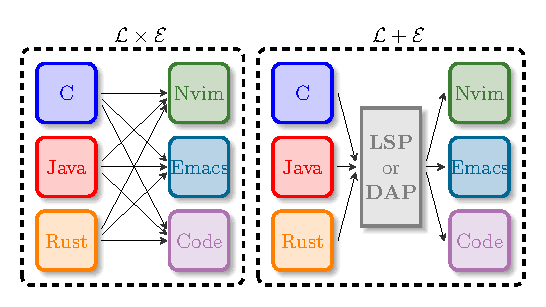
\includegraphics[width=0.9\linewidth]{figs/concept/lsp_combinations.pdf}
    \caption{Traditional approach vs LSP/DAP approach to language support.}
    \label{lst:concept:lsp_combinations}
\end{figure}

As shown in Figure~\ref{lst:concept:lsp_combinations}, the traditional approach to language support requires a separate implementation for each language, resulting in a combinatorial explosion of implementations. In contrast, the Language Server Protocol (LSP) and Debug Adapter Protocol (DAP) provide a standardized interface that decouples the language server from the client, allowing a single language server to support multiple languages. This approach significantly reduces the number of required implementations, simplifying the development and maintenance of language servers.
In our approach, we aim to further reduce the number of required implementations by introducing a \textbf{client generator} that automatically generates client code for a given language bringing the number of required implementations to $\mathcal{L} \times 1$.
Currently, there are lots of \textit{editor}, such as \textit{Visual Studio Code}, \textit{Vim/Nvim}, \textit{Emacs} and \textit{IntelliJ IDEA}, that support the LSP and DAP protocols. The client generator will be able to generate the client code for these editors, allowing the language server to be used with any of them.

\subsection{Syntax Highlighting Generator}\label{subsec:concept:SyntaxHighlightingGenerator}

One of the key components of a modern code editor is syntax highlighting. Proper syntax highlighting significantly enhances the readability and maintainability of code by visually distinguishing elements such as keywords, operators, strings, and comments. In our approach, we have developed a sophisticated \textbf{Syntax Highlighting Generator} that receive in input the keywords and other syntactic elements from a given language specification and generates the corresponding syntax highlighting configuration for various editors.

By parsing the language's grammar and lexical rules, the parser gets keywords, operators, and other syntactic constructs. The generator then maps these elements to appropriate highlighting rules for each supported editor. This process ensures that syntax highlighting is both accurate and consistent across different editors.

Our generator supports a wide range of editors, including Visual Studio Code, Vim/Nvim, Emacs. For each editor, the generator produces a configuration file or plugin that can be easily integrated into the editor's ecosystem. This automation not only saves significant development time but also ensures that the syntax highlighting is always up-to-date with the latest language specifications.

Moreover, the Syntax Highlighting Generator is highly customizable. Developers can specify additional highlighting rules or override the default behavior to accommodate specific needs. This flexibility makes our generator suitable for both general-purpose programming languages and domain-specific languages (DSLs).

In summary, our Syntax Highlighting Generator streamlines the process of creating and maintaining syntax highlighting configurations. By automating this task, we ensure that developers can focus on writing code rather than manually configuring their editors. The result is a more efficient and enjoyable coding experience, regardless of the chosen editor.

\subsection{LSP Generation}\label{subsec:concept:LSPGeneration}

The Language Server Protocol (LSP) has revolutionized the way code editors and IDEs provide language-specific features such as auto-completion, go-to-definition, and refactoring. However, creating an LSP server from scratch for each language can still be a daunting task. To address this challenge, we have developed a comprehensive \textbf{LSP Generation} framework that simplifies the creation of LSP servers.

Our LSP Generation framework leverages the language specification to automatically generate the boilerplate code required for an LSP server. This includes setting up the communication protocol, handling initialization, and managing language-specific requests and notifications. By automating these aspects, our framework significantly reduces the amount of manual coding required to implement an LSP server.

The core of our LSP Generation framework is a set of templates and code generation tools that can be customized for different languages. These templates include common LSP server components such as text document synchronization, hover information, and diagnostics. Developers can extend these templates to support additional language features or integrate with existing tools and libraries.

Our framework also includes a comprehensive test suite to ensure the generated LSP server is compliant with the LSP specification and performs reliably. This suite includes unit tests for individual components as well as integration tests that simulate common usage scenarios. By providing a robust testing infrastructure, we help developers deliver high-quality LSP servers with confidence.

One of the key advantages of our LSP Generation framework is its extensibility. Developers can easily add support for new languages or customize existing templates to meet their specific requirements. This flexibility ensures that our framework can evolve with the ever-changing landscape of programming languages and development tools.

Overall, our LSP Generation framework represents a significant advancement in the development of language servers. By automating much of the boilerplate code and providing a robust testing infrastructure, we enable developers to quickly and efficiently create high-quality LSP servers. This reduces the overall development effort and accelerates the adoption of the LSP across different languages and editors.

\subsection{Client Generator}\label{subsec:concept:ClientGenerator}

The heart of our innovative approach lies in the \textbf{Client Generator}, a powerful tool designed to automatically generate client code for various editors, thereby reducing the number of required implementations to $\mathbf{L} \times 1$. This remarkable reduction in effort and complexity is achieved through a combination of advanced templating, code analysis, and generation techniques.

\begin{enumerate}
\item The Client Generator works by taking a language specification as input and producing the necessary client code for editors that support the LSP and DAP protocols. This process involves several steps:
\item Language Analysis: The generator analyzes the language specification to identify key constructs such as syntax rules, semantic rules, and debugging capabilities. This information is used to tailor the generated client code to the specific needs of the language.
\item Template Customization: Based on the language analysis, the generator customizes a set of pre-defined templates for each supported editor. These templates include code for initializing the client, handling LSP and DAP requests, and integrating with the editor's ecosystem.
\item Code Generation: The customized templates are then used to generate the client code. This code is structured to be easily maintainable and extensible, allowing developers to further customize it if needed.
\item Integration and Testing: The generated client code is integrated with the target editors and subjected to a rigorous testing process. This includes both automated tests and manual verification to ensure the generated code works seamlessly with the language server and provides a smooth user experience.
\end{enumerate}

By automating the generation of client code, our Client Generator dramatically reduces the time and effort required to support new languages in multiple editors. This not only simplifies the development process but also ensures a consistent and high-quality experience for users across different editors.

\subsection{Modular Reuse and Reduction to $N \times 1$} \label{subsec:concept:ModularReuseAndReductionToNtimes1}

An even more groundbreaking aspect of our approach is the shift from $\mathbf{L} \times 1$ to $\mathbf{N} \times 1$, where $\mathbf{N}$ is significantly less than $\mathbf{L}$. This incredible reduction is made possible by the modular design of our tools, which allows components developed for one language to be reused across multiple other languages.

This modularity is a game-changer. Components such as syntax highlighting rules, LSP implementations, and debugging configurations can be shared and reused, drastically cutting down the number of unique implementations needed. When a new language is introduced, it can often leverage existing components, requiring only minor modifications or extensions. This reuse is facilitated by the interoperability of our generated modules, ensuring that the core functionalities are consistent and reliable across different languages and editors.

For example, if a new language shares similar syntactic or semantic structures with an existing one, the syntax highlighting and LSP components from the existing language can be quickly adapted and reused. This reuse extends beyond mere code copying; our system is designed to recognize and integrate these components seamlessly, ensuring that updates and improvements to shared components propagate across all languages that use them.

This modular reuse also means that the effort to introduce and support a new language is significantly reduced. Instead of starting from scratch, developers can build on a robust foundation of existing components, focusing their efforts on the unique aspects of the new language. This not only accelerates the development process but also ensures a high level of quality and consistency.

In conclusion, the combination of our Syntax Highlighting Generator, LSP Generation framework, Client Generator, and the modular reuse of components represents a transformative approach to language support. By reducing the number of required implementations from $\mathbf{L} \times 1$ to $\mathbf{N} \times 1$, we achieve unparalleled efficiency and flexibility. This innovative approach allows us to rapidly support new languages, maintain high standards of quality, and provide a seamless and consistent user experience across different editors. Our work is not just a technical achievement but a significant step forward in the evolution of development tools, setting new standards for efficiency and modularity in the software industry.

